%!TEX root = ../index.tex
In diesem Kapitel wird die Situation der allink vor Aufnahme dieser Semesterarbeit beschrieben. Das Diagramm in Abbildung~\ref{fig:systemlandschaft} zeigt alle bei allink benutzten Informationssysteme.
\begin{figure}[h]
  \centering
	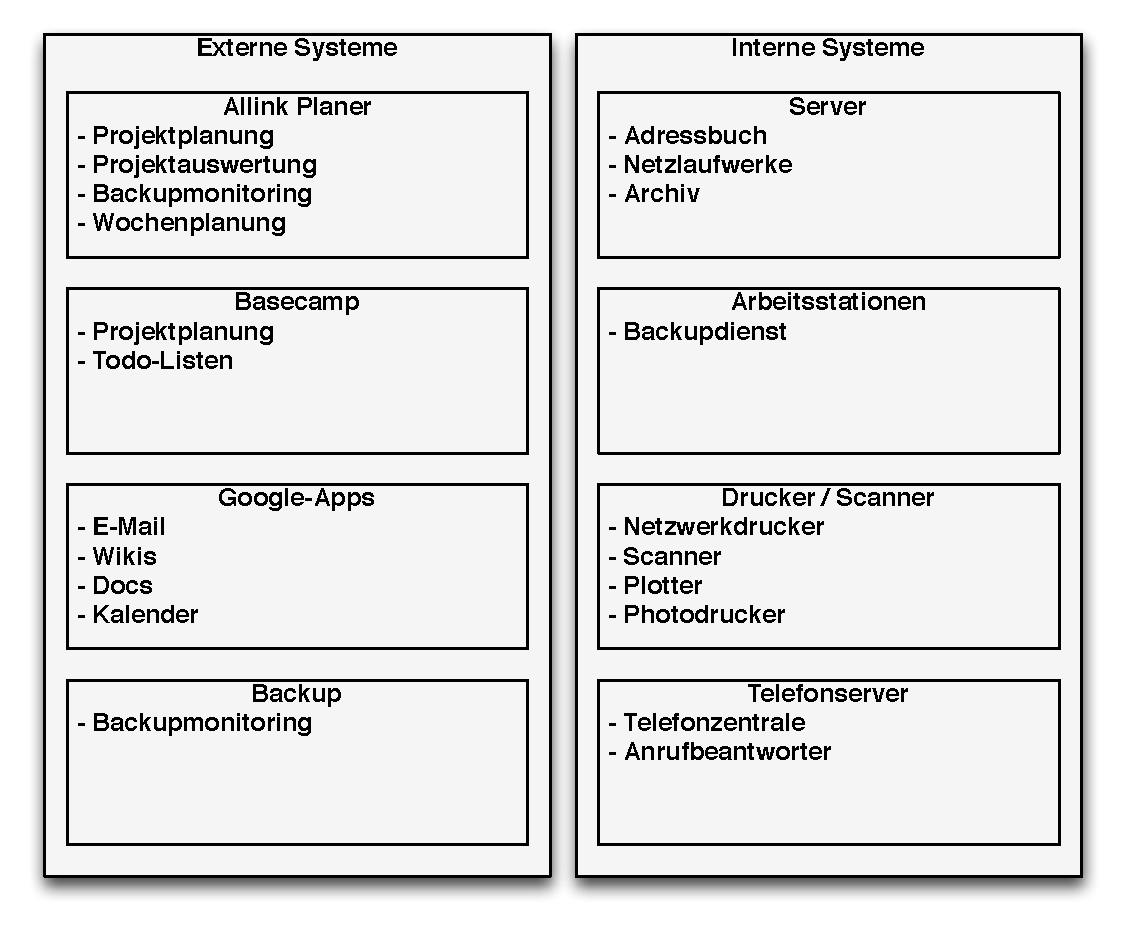
\includegraphics[width=1\textwidth]{include/systemlandschaft.pdf}
	\caption{IT-Systeme in der allink}
	\label{fig:systemlandschaft}
\end{figure}


\section{Systeme mit Benutzermanagement}
\label{sec:Systeme mit Benutzermanagement}
Viele Systeme welche in der allink verwendet werden, sind nicht für die Verwendung als Single-Sign-On System geeignet. So hat zum Beispiel der Telefon Server sehr wohl Benutzerkonten, jedoch sind diese in den Telefon Handgeräten durch die Informatik konfiguriert und die meisten Mitarbeiter wissen somit nicht, dass sie ein Benutzername und ein Passwort für den Telefondienst besitzen. Nachfolgend wird auf drei Systeme eingegangen welche von den Mitarbeitern bewusst verwendet werden und über eine Benutzerverwaltung verfügen.

\subsection{Google Apps}
\label{subs:Google_Apps}
allink verwendet aus Google Apps folgende Tools. 
\begin{itemize}
	\item Google Mail 
	\item Google Calendar 
	\item Google Sites 
	\item Google Docs 
	\item Google Analytics 
\end{itemize}
Google Apps sind bei allink schon seit mehreren Jahren im Einsatz. Google Docs hat Microsoft Office für den internen Gebrauch vollständig abgelöst.

\subsection{Basecamp}
\label{subs:Basecamp}
Mit Basecamp werden Milestones und Todo-Listen für sämtliche Projekte verwaltet. Zudem werden sämtliche Arbeitsaufwände darin erfasst um am Ende eines Projekts einen Überblick über alle Arbeitsleistungen zu haben. Basecamp ist seit mehr als zwei Jahren im Einsatz, wird jedoch nicht von allen Mitarbeitern konsequent genutzt.

\subsection{Mac OS X Server}
\label{subs:Mac OS X Server}
Allink verwendet ausschliesslich Desktop und Notebook Computer der Marke Apple. Für die zentrale Dateiablage wird ein Mac Mini verwendet, auf welchem neben der Dateiablage auch noch ein Adress-Server und weitere Dienste laufen. Die meisten Dienste welche ursprünglich auch auf diesem Server liefen, wurden durch Dienste von Google Apps ersetzt.

\section{Mitarbeiter}
\label{sec:Mitarbeiter}
Da die Mitarbeiter von allink die zukünftigen Benutzer des zu entwickelnden Systems sein werden, wurden 11 Mitarbeiter befragt, welche Passwörter und Logindaten ihnen bekannt sind. Aus den Resultaten der Befragung, welche in Tabelle~\ref{tab:umfrage_passworter} zu sehen sind, geht hervor, dass die meisten Benutzer ihre Logindaten für Google Apps auswendig kennen und nur wenige Mitarbeiter sich bewusst sind, dass sie auf dem zentralen Fileserver ein Konto besitzen.

\begin{table}
  \centering
  \begin{tabular}
  	{|l | c|} \hline System & Anzahl\\
  	\hline Google Apps & 10\\
  	\hline Basecamp & 5\\
  	\hline Mac OS X Server & 4\\
  	\hline 
  \end{tabular}
  \caption{Anzahl Mitarbeiter welche ihre Logindaten kennen}
  \label{tab:umfrage_passworter}
\end{table}

\section{Login Prozess}
\label{sec:Login Prozess}
Die meisten Mitarbeiter kennen nicht die Passwörter sämtlicher Webapplikationen. Darum ist ein zeitraubendes Nachfragen der Daten notwendig falls man nicht mehr eingeloggt ist. Eine Darstellung dieses Vorgehens ist in Abbildung~\ref{fig:login-before} zu sehen.

\begin{figure}
		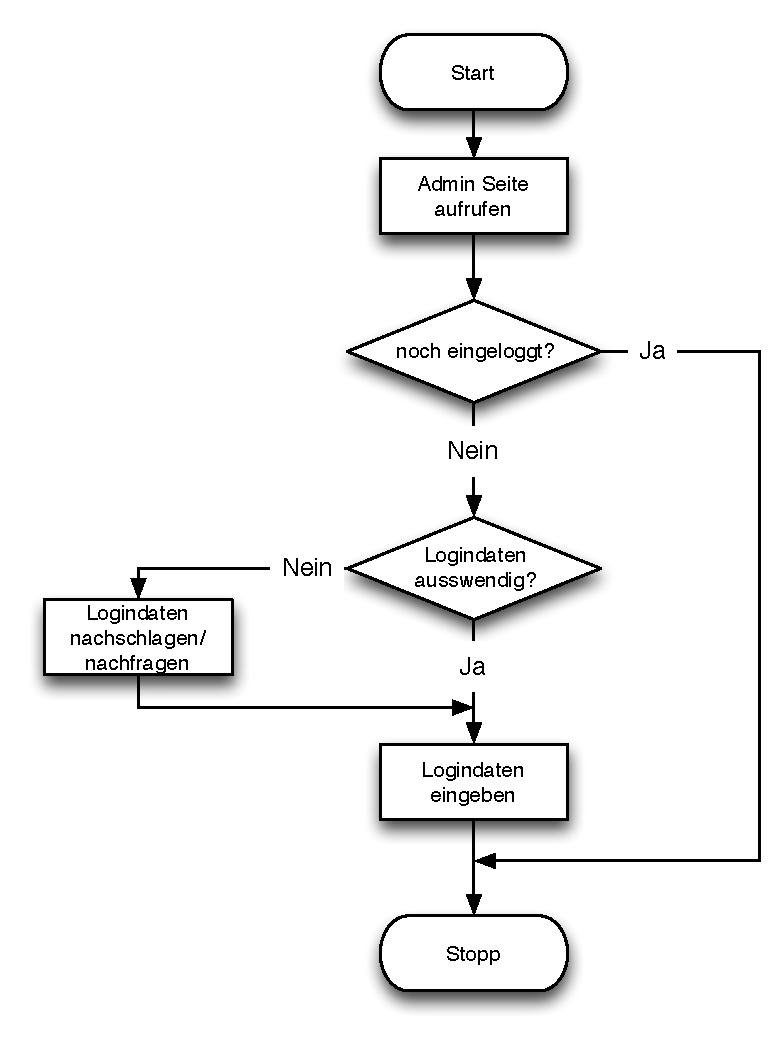
\includegraphics[width=0.70\textwidth]{include/login_before.pdf}
		\caption{Login Prozess vor dieser Arbeit}
		\label{fig:login-before}
\end{figure}
